% Options for packages loaded elsewhere
\PassOptionsToPackage{unicode}{hyperref}
\PassOptionsToPackage{hyphens}{url}
%
\documentclass[
]{article}
\usepackage{amsmath,amssymb}
\usepackage{lmodern}
\usepackage{ifxetex,ifluatex}
\ifnum 0\ifxetex 1\fi\ifluatex 1\fi=0 % if pdftex
  \usepackage[T1]{fontenc}
  \usepackage[utf8]{inputenc}
  \usepackage{textcomp} % provide euro and other symbols
\else % if luatex or xetex
  \usepackage{unicode-math}
  \defaultfontfeatures{Scale=MatchLowercase}
  \defaultfontfeatures[\rmfamily]{Ligatures=TeX,Scale=1}
\fi
% Use upquote if available, for straight quotes in verbatim environments
\IfFileExists{upquote.sty}{\usepackage{upquote}}{}
\IfFileExists{microtype.sty}{% use microtype if available
  \usepackage[]{microtype}
  \UseMicrotypeSet[protrusion]{basicmath} % disable protrusion for tt fonts
}{}
\makeatletter
\@ifundefined{KOMAClassName}{% if non-KOMA class
  \IfFileExists{parskip.sty}{%
    \usepackage{parskip}
  }{% else
    \setlength{\parindent}{0pt}
    \setlength{\parskip}{6pt plus 2pt minus 1pt}}
}{% if KOMA class
  \KOMAoptions{parskip=half}}
\makeatother
\usepackage{xcolor}
\IfFileExists{xurl.sty}{\usepackage{xurl}}{} % add URL line breaks if available
\IfFileExists{bookmark.sty}{\usepackage{bookmark}}{\usepackage{hyperref}}
\hypersetup{
  pdftitle={Data Management with Tidyverse},
  pdfauthor={Cheng Peng},
  hidelinks,
  pdfcreator={LaTeX via pandoc}}
\urlstyle{same} % disable monospaced font for URLs
\usepackage[margin=1in]{geometry}
\usepackage{color}
\usepackage{fancyvrb}
\newcommand{\VerbBar}{|}
\newcommand{\VERB}{\Verb[commandchars=\\\{\}]}
\DefineVerbatimEnvironment{Highlighting}{Verbatim}{commandchars=\\\{\}}
% Add ',fontsize=\small' for more characters per line
\usepackage{framed}
\definecolor{shadecolor}{RGB}{248,248,248}
\newenvironment{Shaded}{\begin{snugshade}}{\end{snugshade}}
\newcommand{\AlertTok}[1]{\textcolor[rgb]{0.94,0.16,0.16}{#1}}
\newcommand{\AnnotationTok}[1]{\textcolor[rgb]{0.56,0.35,0.01}{\textbf{\textit{#1}}}}
\newcommand{\AttributeTok}[1]{\textcolor[rgb]{0.77,0.63,0.00}{#1}}
\newcommand{\BaseNTok}[1]{\textcolor[rgb]{0.00,0.00,0.81}{#1}}
\newcommand{\BuiltInTok}[1]{#1}
\newcommand{\CharTok}[1]{\textcolor[rgb]{0.31,0.60,0.02}{#1}}
\newcommand{\CommentTok}[1]{\textcolor[rgb]{0.56,0.35,0.01}{\textit{#1}}}
\newcommand{\CommentVarTok}[1]{\textcolor[rgb]{0.56,0.35,0.01}{\textbf{\textit{#1}}}}
\newcommand{\ConstantTok}[1]{\textcolor[rgb]{0.00,0.00,0.00}{#1}}
\newcommand{\ControlFlowTok}[1]{\textcolor[rgb]{0.13,0.29,0.53}{\textbf{#1}}}
\newcommand{\DataTypeTok}[1]{\textcolor[rgb]{0.13,0.29,0.53}{#1}}
\newcommand{\DecValTok}[1]{\textcolor[rgb]{0.00,0.00,0.81}{#1}}
\newcommand{\DocumentationTok}[1]{\textcolor[rgb]{0.56,0.35,0.01}{\textbf{\textit{#1}}}}
\newcommand{\ErrorTok}[1]{\textcolor[rgb]{0.64,0.00,0.00}{\textbf{#1}}}
\newcommand{\ExtensionTok}[1]{#1}
\newcommand{\FloatTok}[1]{\textcolor[rgb]{0.00,0.00,0.81}{#1}}
\newcommand{\FunctionTok}[1]{\textcolor[rgb]{0.00,0.00,0.00}{#1}}
\newcommand{\ImportTok}[1]{#1}
\newcommand{\InformationTok}[1]{\textcolor[rgb]{0.56,0.35,0.01}{\textbf{\textit{#1}}}}
\newcommand{\KeywordTok}[1]{\textcolor[rgb]{0.13,0.29,0.53}{\textbf{#1}}}
\newcommand{\NormalTok}[1]{#1}
\newcommand{\OperatorTok}[1]{\textcolor[rgb]{0.81,0.36,0.00}{\textbf{#1}}}
\newcommand{\OtherTok}[1]{\textcolor[rgb]{0.56,0.35,0.01}{#1}}
\newcommand{\PreprocessorTok}[1]{\textcolor[rgb]{0.56,0.35,0.01}{\textit{#1}}}
\newcommand{\RegionMarkerTok}[1]{#1}
\newcommand{\SpecialCharTok}[1]{\textcolor[rgb]{0.00,0.00,0.00}{#1}}
\newcommand{\SpecialStringTok}[1]{\textcolor[rgb]{0.31,0.60,0.02}{#1}}
\newcommand{\StringTok}[1]{\textcolor[rgb]{0.31,0.60,0.02}{#1}}
\newcommand{\VariableTok}[1]{\textcolor[rgb]{0.00,0.00,0.00}{#1}}
\newcommand{\VerbatimStringTok}[1]{\textcolor[rgb]{0.31,0.60,0.02}{#1}}
\newcommand{\WarningTok}[1]{\textcolor[rgb]{0.56,0.35,0.01}{\textbf{\textit{#1}}}}
\usepackage{graphicx}
\makeatletter
\def\maxwidth{\ifdim\Gin@nat@width>\linewidth\linewidth\else\Gin@nat@width\fi}
\def\maxheight{\ifdim\Gin@nat@height>\textheight\textheight\else\Gin@nat@height\fi}
\makeatother
% Scale images if necessary, so that they will not overflow the page
% margins by default, and it is still possible to overwrite the defaults
% using explicit options in \includegraphics[width, height, ...]{}
\setkeys{Gin}{width=\maxwidth,height=\maxheight,keepaspectratio}
% Set default figure placement to htbp
\makeatletter
\def\fps@figure{htbp}
\makeatother
\setlength{\emergencystretch}{3em} % prevent overfull lines
\providecommand{\tightlist}{%
  \setlength{\itemsep}{0pt}\setlength{\parskip}{0pt}}
\setcounter{secnumdepth}{5}
\ifluatex
  \usepackage{selnolig}  % disable illegal ligatures
\fi

\title{Data Management with Tidyverse}
\author{Cheng Peng}
\date{}

\begin{document}
\maketitle

{
\setcounter{tocdepth}{4}
\tableofcontents
}
\hypertarget{introduction}{%
\section{Introduction}\label{introduction}}

Data visualization is a form of data analysis (also called visual
analytics). This means we need to prepare data for the visualization.

The major data management tasks are data aggregation and extraction.

\begin{itemize}
\item
  \textbf{Information Aggregation} - combining information in different
  relational data sets to make a integrated single data set for data
  visualization.
\item
  \textbf{Information Extraction} - subsetting a single data set to make
  small data sets that have specific information for creating a
  visualization.
\end{itemize}

The base R package has some powerful and easy to use functions to
perform these types of data management.

\hypertarget{data-cleaning-and-preparation-for-visualization}{%
\section{Data Cleaning and Preparation for
Visualization}\label{data-cleaning-and-preparation-for-visualization}}

\hypertarget{data-cleaning}{%
\subsection{Data Cleaning}\label{data-cleaning}}

Data cleaning refers the process of making a data set possibly from
different sources of \texttt{raw\ data} for modeling, visualization and
relevant analysis. The major tasks include:

\begin{itemize}
\tightlist
\item
  Removing unnecessary variables
\item
  Deleting duplicate rows/observations
\item
  Addressing outliers or invalid data
\item
  Dealing with missing values
\item
  Standardizing or categorizing values
\item
  Correcting typographical errors
\end{itemize}

\hypertarget{data-preparation-for-visualization}{%
\subsection{Data Preparation for
Visualization}\label{data-preparation-for-visualization}}

For a specific data analysis such as modeling or data visualization, we
need to create an analytic data set based on clean data sets.

\textbf{Formating/Conversion}

\begin{itemize}
\tightlist
\item
  Formatting columns appropriately (numbers are treated as numbers,
  dates as dates)
\item
  Convert values into appropriate units
\end{itemize}

\textbf{Filtering/Fubsetting}

\begin{itemize}
\tightlist
\item
  Filter your data to focus on the specific data that interests you.
\item
  Group data and create aggregate values for groups (Counts, Min, Max,
  Mean, Median, Mode)
\item
  Extract values from complex columns
\end{itemize}

\textbf{Aggregation/Merging}

\begin{itemize}
\tightlist
\item
  Combine variables to create new columns
\item
  Merge different relational data sets
\end{itemize}

\hypertarget{r-tools-for-basic-data-management}{%
\section{R Tools For Basic Data
Management}\label{r-tools-for-basic-data-management}}

There are different packages in R have various functions capable of
doing data management. In this note, we introduce the commonly used
functions in base R and in \texttt{tydyverse}.

\hypertarget{merge-data-sets}{%
\subsection{Merge Data Sets}\label{merge-data-sets}}

It is very common that the information we are interested in resides in
different data sources. In order to merge different data sets, there
must be at least one variable ``key'' that links to different data sets.

\begin{Shaded}
\begin{Highlighting}[]
\FunctionTok{include\_graphics}\NormalTok{(}\StringTok{"https://github.com/pengdsci/sta553/raw/main/DataManagement/joins.png"}\NormalTok{)}
\end{Highlighting}
\end{Shaded}

\begin{center}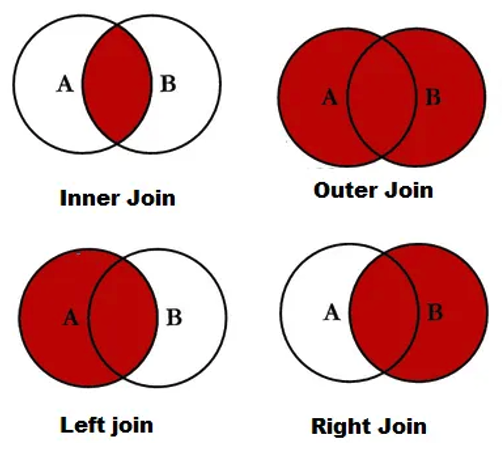
\includegraphics[width=5px,height=5]{https://github.com/pengdsci/sta553/raw/main/DataManagement/joins} \end{center}

\hypertarget{overview-of-tydyverse}{%
\section{Overview of Tydyverse}\label{overview-of-tydyverse}}

There several R libraries that have powerful tool for data wrangling and
information extraction. Tidyverse is a collection of essential R
packages for data science. There 8 packages under the
\texttt{tidyverse\ umbrella} that help us in performing and interacting
with the data.

\hypertarget{packages-for-data-wrangling-and-transformation}{%
\subsection{Packages for Data Wrangling and
Transformation}\label{packages-for-data-wrangling-and-transformation}}

\begin{itemize}
\item
  \textbf{dplyr} provides helper tools for the most common data
  manipulation tasks. It is built to work directly with data frames and
  has the ability to work directly with data stored in an external
  database. We can conduct queries on the database directly, and pull
  back into R only what we need for analysis.
\item
  \textbf{tidyr} addresses the common problem of wanting to reshape the
  data with sophisticated layout for plotting and usage by different R
  functions.
\item
  \textbf{stringr} deals with string variables. It plays a big role in
  processing raw data into a cleaner and an easily understandable
  format.
\item
  \textbf{forcats} is dedicated to dealing with categorical variables or
  factors. Anyone who has worked with categorical data knows what a
  nightmare they can be.
\end{itemize}

\hypertarget{pacakges-for-data-import-and-management}{%
\subsection{Pacakges for Data Import and
Management}\label{pacakges-for-data-import-and-management}}

\begin{itemize}
\item
  \textbf{tibble} is a new modern data frame with nicer behavior around
  printing, subsetting, and factor handling. It keeps many important
  features of the original data frame and removes many of the outdated
  features.
\item
  \textbf{readr} package is recently developed to deal with reading in
  large flat files quickly. The package provides replacements for
  functions like read.table() and read.csv(). The analogous functions in
  readr are read\_table() and read\_csv().
\end{itemize}

\hypertarget{functional-programming-with-library-purrr}{%
\subsection{\texorpdfstring{Functional Programming with Library
\textbf{\{purrr\}}}{Functional Programming with Library \{purrr\}}}\label{functional-programming-with-library-purrr}}

\begin{itemize}
\tightlist
\item
  \textbf{purrr} is a new package that fills in the missing pieces in
  R's functional programming tools. This is not a coding class. We will
  not use Purrr in this class.
\end{itemize}

\hypertarget{data-visualization-and-exploration}{%
\subsection{Data Visualization and
Exploration}\label{data-visualization-and-exploration}}

\textbf{ggplot2} is a powerful and a flexible R package for producing
elegant graphics. The concept behind \texttt{ggplot2} divides plot into
three different fundamental parts:
\texttt{Plot\ =\ data\ +\ Aesthetics\ +\ Geometry}.

The principal components of every plot can be defined as follow:

\begin{itemize}
\item
  \textbf{Aesthetics} is used to indicate x and y variables. It can also
  be used to control the color, the size or the shape of points, the
  height of bars, etc.
\item
  \textbf{Geometry} defines the type of graphics (histogram, box plot,
  line plot, density plot, dot plot, etc.)
\end{itemize}

This will be one of the primary tools for this class.

\hypertarget{data-management-with-dplyr}{%
\section{\texorpdfstring{Data Management with
\texttt{dplyr}}{Data Management with dplyr}}\label{data-management-with-dplyr}}

What we can do in the standard SQL can also be done with \texttt{dyplr}.
For the convenience of illustration, we use a simple well-known built-in
\texttt{iris\ data\ set}.

\hypertarget{pipe-operator}{%
\subsection{\texorpdfstring{Pipe Operator
\texttt{\%\textgreater{}\%}}{Pipe Operator \%\textgreater\%}}\label{pipe-operator}}

The pipe operator, written as \texttt{\%\textgreater{}\%} takes the
output of one function and passes it into another function as an
argument. This allows us to link a sequence of analysis steps using
functions in \texttt{dplyr} and \texttt{tidyr} in data wrangling.

\begin{Shaded}
\begin{Highlighting}[]
\FunctionTok{data}\NormalTok{(iris)}
\FunctionTok{str}\NormalTok{(iris)}
\end{Highlighting}
\end{Shaded}

\begin{verbatim}
## 'data.frame':    150 obs. of  5 variables:
##  $ Sepal.Length: num  5.1 4.9 4.7 4.6 5 5.4 4.6 5 4.4 4.9 ...
##  $ Sepal.Width : num  3.5 3 3.2 3.1 3.6 3.9 3.4 3.4 2.9 3.1 ...
##  $ Petal.Length: num  1.4 1.4 1.3 1.5 1.4 1.7 1.4 1.5 1.4 1.5 ...
##  $ Petal.Width : num  0.2 0.2 0.2 0.2 0.2 0.4 0.3 0.2 0.2 0.1 ...
##  $ Species     : Factor w/ 3 levels "setosa","versicolor",..: 1 1 1 1 1 1 1 1 1 1 ...
\end{verbatim}

\hypertarget{common-dplyr-functions}{%
\subsection{\texorpdfstring{Common \texttt{dplyr}
Functions}{Common dplyr Functions}}\label{common-dplyr-functions}}

The following is the list of functions in \texttt{dplyr}.

\begin{itemize}
\tightlist
\item
  \textbf{select()}: sub-setting columns.
\end{itemize}

To select columns of a data frame, use \texttt{select()}. The first
argument to this function is the data frame (\texttt{iris}), and the
subsequent arguments are the columns to keep. For example

\begin{Shaded}
\begin{Highlighting}[]
\NormalTok{iris.petal }\OtherTok{=} \FunctionTok{select}\NormalTok{(iris, Petal.Length, Petal.Width, Species)}
\FunctionTok{str}\NormalTok{(iris.petal)}
\end{Highlighting}
\end{Shaded}

\begin{verbatim}
## 'data.frame':    150 obs. of  3 variables:
##  $ Petal.Length: num  1.4 1.4 1.3 1.5 1.4 1.7 1.4 1.5 1.4 1.5 ...
##  $ Petal.Width : num  0.2 0.2 0.2 0.2 0.2 0.4 0.3 0.2 0.2 0.1 ...
##  $ Species     : Factor w/ 3 levels "setosa","versicolor",..: 1 1 1 1 1 1 1 1 1 1 ...
\end{verbatim}

To select all columns except certain ones, put a ``-'' in front of the
variable to exclude it. For example, we \textbf{exclude} Petal
information and only \textbf{keep} Sepal information, we can use the
following code

\begin{Shaded}
\begin{Highlighting}[]
\NormalTok{iris.sepal }\OtherTok{=} \FunctionTok{select}\NormalTok{(iris, }\SpecialCharTok{{-}}\NormalTok{Petal.Length, }\SpecialCharTok{{-}}\NormalTok{Petal.Width)}
\FunctionTok{str}\NormalTok{(iris.sepal)}
\end{Highlighting}
\end{Shaded}

\begin{verbatim}
## 'data.frame':    150 obs. of  3 variables:
##  $ Sepal.Length: num  5.1 4.9 4.7 4.6 5 5.4 4.6 5 4.4 4.9 ...
##  $ Sepal.Width : num  3.5 3 3.2 3.1 3.6 3.9 3.4 3.4 2.9 3.1 ...
##  $ Species     : Factor w/ 3 levels "setosa","versicolor",..: 1 1 1 1 1 1 1 1 1 1 ...
\end{verbatim}

This will select all the variables in surveys except for
\texttt{Petal.Length}, and \texttt{Petal.Width}.

\begin{itemize}
\tightlist
\item
  \textbf{filter()}: sub-setting rows on conditions.
\end{itemize}

For example, if we only select one species \texttt{versicolor}, we can
use the following code.

\begin{Shaded}
\begin{Highlighting}[]
\NormalTok{versicolor }\OtherTok{=} \FunctionTok{filter}\NormalTok{(iris, Species }\SpecialCharTok{==}\StringTok{"versicolor"}\NormalTok{)}
\FunctionTok{summary}\NormalTok{(versicolor)}
\end{Highlighting}
\end{Shaded}

\begin{verbatim}
##   Sepal.Length    Sepal.Width     Petal.Length   Petal.Width          Species  
##  Min.   :4.900   Min.   :2.000   Min.   :3.00   Min.   :1.000   setosa    : 0  
##  1st Qu.:5.600   1st Qu.:2.525   1st Qu.:4.00   1st Qu.:1.200   versicolor:50  
##  Median :5.900   Median :2.800   Median :4.35   Median :1.300   virginica : 0  
##  Mean   :5.936   Mean   :2.770   Mean   :4.26   Mean   :1.326                  
##  3rd Qu.:6.300   3rd Qu.:3.000   3rd Qu.:4.60   3rd Qu.:1.500                  
##  Max.   :7.000   Max.   :3.400   Max.   :5.10   Max.   :1.800
\end{verbatim}

If we subset a data set by select certain number of columns and row with
multiple conditions, pipe operator \texttt{\%\textgreater{}\%} will make
subsetting easy. For example, if we only want to study
\texttt{sepal\ width} and \texttt{length} of \texttt{setosa} where petal
length is less than 1.5. The following code using
\texttt{\%\textgreater{}\%}

\begin{Shaded}
\begin{Highlighting}[]
\NormalTok{resulting.subset }\OtherTok{\textless{}{-}}\NormalTok{ iris }\SpecialCharTok{\%\textgreater{}\%}
             \FunctionTok{filter}\NormalTok{(Petal.Length }\SpecialCharTok{\textless{}} \FloatTok{1.5}\NormalTok{, Species }\SpecialCharTok{==}\StringTok{"setosa"}\NormalTok{) }\SpecialCharTok{\%\textgreater{}\%}
             \FunctionTok{select}\NormalTok{(Sepal.Length, Sepal.Width, Species)}
\FunctionTok{summary}\NormalTok{(resulting.subset)}
\end{Highlighting}
\end{Shaded}

\begin{verbatim}
##   Sepal.Length    Sepal.Width          Species  
##  Min.   :4.300   Min.   :2.300   setosa    :24  
##  1st Qu.:4.600   1st Qu.:3.000   versicolor: 0  
##  Median :4.900   Median :3.350   virginica : 0  
##  Mean   :4.896   Mean   :3.333                  
##  3rd Qu.:5.100   3rd Qu.:3.525                  
##  Max.   :5.800   Max.   :4.200
\end{verbatim}

Note that, multiple conditional statements are separated by \texttt{,}
or \texttt{\&}. Using \texttt{\%\textgreater{}\%}, we don't need to
include the data set as the first argument.

\begin{itemize}
\tightlist
\item
  \textbf{mutate()}: creating new columns by using information from
  other columns.
\end{itemize}

Frequently we want to create new columns based on the values in existing
columns. For example, we want to define two ratios of the sepal and
petal widths and sepal and petal lengths. For this we'll use mutate().

\begin{Shaded}
\begin{Highlighting}[]
\NormalTok{expanded.data }\OtherTok{\textless{}{-}}\NormalTok{ iris }\SpecialCharTok{\%\textgreater{}\%}
             \FunctionTok{mutate}\NormalTok{(}\AttributeTok{length.ratio =}\NormalTok{ Sepal.Length}\SpecialCharTok{/}\NormalTok{Petal.Length,}
                    \AttributeTok{width.ratio =}\NormalTok{ Sepal.Width}\SpecialCharTok{/}\NormalTok{Petal.Width)}
\FunctionTok{summary}\NormalTok{(expanded.data)}
\end{Highlighting}
\end{Shaded}

\begin{verbatim}
##   Sepal.Length    Sepal.Width     Petal.Length    Petal.Width   
##  Min.   :4.300   Min.   :2.000   Min.   :1.000   Min.   :0.100  
##  1st Qu.:5.100   1st Qu.:2.800   1st Qu.:1.600   1st Qu.:0.300  
##  Median :5.800   Median :3.000   Median :4.350   Median :1.300  
##  Mean   :5.843   Mean   :3.057   Mean   :3.758   Mean   :1.199  
##  3rd Qu.:6.400   3rd Qu.:3.300   3rd Qu.:5.100   3rd Qu.:1.800  
##  Max.   :7.900   Max.   :4.400   Max.   :6.900   Max.   :2.500  
##        Species    length.ratio    width.ratio    
##  setosa    :50   Min.   :1.050   Min.   : 1.130  
##  versicolor:50   1st Qu.:1.230   1st Qu.: 1.603  
##  virginica :50   Median :1.411   Median : 2.148  
##                  Mean   :2.018   Mean   : 6.628  
##                  3rd Qu.:3.176   3rd Qu.:11.583  
##                  Max.   :4.833   Max.   :41.000
\end{verbatim}

\begin{itemize}
\tightlist
\item
  \textbf{group\_by()} and \textbf{summarize()}: creating summary
  statistics on grouped data.
\end{itemize}

group\_by() is often used together with summarize(), which collapses
each group into a single-row summary of that group. group\_by() takes as
arguments the column names that contain the categorical variables for
which you want to calculate the summary statistics.

The following code yields a set of summarized statistics include mean of
sepal width and and length as well as the correlation coefficients in
each of the three species.

\begin{Shaded}
\begin{Highlighting}[]
\NormalTok{summary.stats }\OtherTok{\textless{}{-}}\NormalTok{ iris }\SpecialCharTok{\%\textgreater{}\%}
             \FunctionTok{group\_by}\NormalTok{(Species) }\SpecialCharTok{\%\textgreater{}\%}
             \FunctionTok{summarize}\NormalTok{(}\AttributeTok{sepal.width.avg =} \FunctionTok{mean}\NormalTok{(Sepal.Width),}
                       \AttributeTok{sepal.length.avg =} \FunctionTok{mean}\NormalTok{(Sepal.Length),}
                       \AttributeTok{corr.sepal =} \FunctionTok{cor}\NormalTok{(Sepal.Length, Sepal.Width)) }
\NormalTok{summary.stats}
\end{Highlighting}
\end{Shaded}

\begin{verbatim}
## # A tibble: 3 x 4
##   Species    sepal.width.avg sepal.length.avg corr.sepal
##   <fct>                <dbl>            <dbl>      <dbl>
## 1 setosa                3.43             5.01      0.743
## 2 versicolor            2.77             5.94      0.526
## 3 virginica             2.97             6.59      0.457
\end{verbatim}

All R functions such as \texttt{min()}, \texttt{max()}, , that yield
summarized statistics can be used with \texttt{summarize()}. We can also
filter out some observations before we compute tge summary statistics.

\begin{Shaded}
\begin{Highlighting}[]
\NormalTok{summary.stats.filtering }\OtherTok{\textless{}{-}}\NormalTok{ iris }\SpecialCharTok{\%\textgreater{}\%}
             \FunctionTok{filter}\NormalTok{(Petal.Length }\SpecialCharTok{\textless{}} \DecValTok{5}\NormalTok{) }\SpecialCharTok{\%\textgreater{}\%}
             \FunctionTok{group\_by}\NormalTok{(Species) }\SpecialCharTok{\%\textgreater{}\%}
             \FunctionTok{summarize}\NormalTok{(}\AttributeTok{sepal.width.avg =} \FunctionTok{mean}\NormalTok{(Sepal.Width),}
                       \AttributeTok{sepal.length.avg =} \FunctionTok{mean}\NormalTok{(Sepal.Length),}
                       \AttributeTok{corr.sepal =} \FunctionTok{cor}\NormalTok{(Sepal.Length, Sepal.Width)) }
\NormalTok{summary.stats.filtering}
\end{Highlighting}
\end{Shaded}

\begin{verbatim}
## # A tibble: 3 x 4
##   Species    sepal.width.avg sepal.length.avg corr.sepal
##   <fct>                <dbl>            <dbl>      <dbl>
## 1 setosa                3.43             5.01      0.743
## 2 versicolor            2.77             5.92      0.519
## 3 virginica             2.8              5.85      0.643
\end{verbatim}

\begin{itemize}
\tightlist
\item
  \textbf{arrange()}: sorting results.
\end{itemize}

To sort in descending order, we need to add the \texttt{desc()}
function. If we want to sort the results by decreasing order of mean
weight.

\begin{Shaded}
\begin{Highlighting}[]
\NormalTok{summary.stats.sort }\OtherTok{\textless{}{-}}\NormalTok{ iris }\SpecialCharTok{\%\textgreater{}\%}
             \FunctionTok{filter}\NormalTok{(Petal.Length }\SpecialCharTok{\textless{}} \DecValTok{5}\NormalTok{) }\SpecialCharTok{\%\textgreater{}\%}
             \FunctionTok{group\_by}\NormalTok{(Species) }\SpecialCharTok{\%\textgreater{}\%}
             \FunctionTok{summarize}\NormalTok{(}\AttributeTok{sepal.width.avg =} \FunctionTok{mean}\NormalTok{(Sepal.Width),}
                       \AttributeTok{sepal.length.avg =} \FunctionTok{mean}\NormalTok{(Sepal.Length),}
                       \AttributeTok{corr.sepal =} \FunctionTok{cor}\NormalTok{(Sepal.Length, Sepal.Width)) }\SpecialCharTok{\%\textgreater{}\%}
              \FunctionTok{arrange}\NormalTok{(}\FunctionTok{desc}\NormalTok{(corr.sepal))}
\NormalTok{summary.stats.sort}
\end{Highlighting}
\end{Shaded}

\begin{verbatim}
## # A tibble: 3 x 4
##   Species    sepal.width.avg sepal.length.avg corr.sepal
##   <fct>                <dbl>            <dbl>      <dbl>
## 1 setosa                3.43             5.01      0.743
## 2 virginica             2.8              5.85      0.643
## 3 versicolor            2.77             5.92      0.519
\end{verbatim}

The resulting data set can also be sorted by multiple variables.

\begin{itemize}
\tightlist
\item
  \textbf{count()}: counting discrete values.
\end{itemize}

When working with data, we often want to know the number of observations
found for each factor or combination of factors. For this task,
\texttt{dplyr} provides \texttt{count()}. For example, if we wanted to
count the number of rows of data for each species after we filter out
all records with Petal Length \textless{} 5, we would do:

\begin{Shaded}
\begin{Highlighting}[]
\NormalTok{summary.count }\OtherTok{\textless{}{-}}\NormalTok{ iris }\SpecialCharTok{\%\textgreater{}\%}
             \FunctionTok{filter}\NormalTok{(Petal.Length }\SpecialCharTok{\textless{}} \DecValTok{5}\NormalTok{) }\SpecialCharTok{\%\textgreater{}\%}
             \FunctionTok{group\_by}\NormalTok{(Species) }\SpecialCharTok{\%\textgreater{}\%}
             \FunctionTok{summarize}\NormalTok{(}\AttributeTok{count =} \FunctionTok{n}\NormalTok{(), }\AttributeTok{sort =} \ConstantTok{TRUE}\NormalTok{) }
\NormalTok{summary.count}
\end{Highlighting}
\end{Shaded}

\begin{verbatim}
## # A tibble: 3 x 3
##   Species    count sort 
##   <fct>      <int> <lgl>
## 1 setosa        50 TRUE 
## 2 versicolor    48 TRUE 
## 3 virginica      6 TRUE
\end{verbatim}

If we wanted to count combination of factors, say \texttt{factor\ A} and
\texttt{factor\ B}, we would specify the first and the second factor as
the arguments of \texttt{count(factor\ A,\ factor\ B)}.

\hypertarget{reshaping-functions-in-tidyr}{%
\subsection{\texorpdfstring{Reshaping Functions in
\texttt{tidyr}}{Reshaping Functions in tidyr}}\label{reshaping-functions-in-tidyr}}

The \texttt{tidyr} package complements \texttt{dplyr} perfectly. It
boosts the power of dplyr for data manipulation and pre-processing. To
illustrate how to use these functions, we consider define a subset from
\texttt{iris} that contains only two variables: Sepal Length and
Species.

\begin{Shaded}
\begin{Highlighting}[]
\NormalTok{life.expectancy }\OtherTok{\textless{}{-}}\FunctionTok{read.csv}\NormalTok{(}\StringTok{"https://stat553.s3.amazonaws.com/Tidyverse/life\_expectancy\_years+.csv"}\NormalTok{)}
\NormalTok{life.expectancy[}\DecValTok{1}\SpecialCharTok{:}\DecValTok{5}\NormalTok{, }\DecValTok{1}\SpecialCharTok{:}\DecValTok{10}\NormalTok{]}
\end{Highlighting}
\end{Shaded}

\begin{verbatim}
##                country X1799 X1800 X1801 X1802 X1803 X1804 X1805 X1806 X1807
## 1          Afghanistan  28.2  28.2  28.2  28.2  28.2  28.2  28.1  28.1  28.1
## 2               Angola  27.0  27.0  27.0  27.0  27.0  27.0  27.0  27.0  27.0
## 3              Albania  35.4  35.4  35.4  35.4  35.4  35.4  35.4  35.4  35.4
## 4              Andorra    NA    NA    NA    NA    NA    NA    NA    NA    NA
## 5 United Arab Emirates  30.7  30.7  30.7  30.7  30.7  30.7  30.7  30.7  30.7
\end{verbatim}

\texttt{sub.iris} is called a \textbf{long table}. We can reshape this
\textbf{long table} to a \textbf{wide table} using \texttt{spread()}
function.

\begin{itemize}
\item
  \textbf{gather()}: The function ``gathers'' multiple columns from the
  data set and converts them into key-value pairs. \texttt{gather()}
  takes four principal arguments:

  \begin{itemize}
  \tightlist
  \item
    data set
  \item
    the key column variable we wish to create from column names.
  \item
    the values column variable we wish to create and fill with values
    associated with the key.
  \end{itemize}
\end{itemize}

\texttt{The\ names\ of\ the\ columns\ we\ use\ to\ fill\ the\ key\ variable\ (or\ to\ drop)}.

Here we exclude \texttt{country} from being \texttt{gather()}ed.

\begin{Shaded}
\begin{Highlighting}[]
\NormalTok{life.expectancy.long }\OtherTok{\textless{}{-}}\NormalTok{ life.expectancy }\SpecialCharTok{\%\textgreater{}\%}
  \FunctionTok{gather}\NormalTok{(}\AttributeTok{key =} \StringTok{"Year"}\NormalTok{,       }\CommentTok{\# the column names of the wide table}
         \AttributeTok{value =} \StringTok{"lifeExp"}\NormalTok{,  }\CommentTok{\# the numerical values of the table}
         \SpecialCharTok{{-}}\NormalTok{ country,          }\CommentTok{\# drop country variable: its value will not be gathered (stacked)!}
         \AttributeTok{na.rm =} \ConstantTok{TRUE}\NormalTok{)       }\CommentTok{\# removing records with missing values}
\DocumentationTok{\#\#}
\FunctionTok{head}\NormalTok{(life.expectancy.long)}
\end{Highlighting}
\end{Shaded}

\begin{verbatim}
##                country  Year lifeExp
## 1          Afghanistan X1799    28.2
## 2               Angola X1799    27.0
## 3              Albania X1799    35.4
## 5 United Arab Emirates X1799    30.7
## 6            Argentina X1799    33.2
## 7              Armenia X1799    34.0
\end{verbatim}

We can use \texttt{substr()} to remove \texttt{X} from variable
\texttt{Year} as shown in the following code.

\begin{Shaded}
\begin{Highlighting}[]
\NormalTok{correct.life.exp.data }\OtherTok{\textless{}{-}}\NormalTok{ life.expectancy.long }\SpecialCharTok{\%\textgreater{}\%}
                      \FunctionTok{mutate}\NormalTok{(}\AttributeTok{year =} \FunctionTok{substr}\NormalTok{(Year,}\DecValTok{2}\NormalTok{,}\DecValTok{5}\NormalTok{)) }\SpecialCharTok{\%\textgreater{}\%}
                      \FunctionTok{select}\NormalTok{(}\SpecialCharTok{{-}}\NormalTok{Year)}
\FunctionTok{head}\NormalTok{(correct.life.exp.data)}
\end{Highlighting}
\end{Shaded}

\begin{verbatim}
##                country lifeExp year
## 1          Afghanistan    28.2 1799
## 2               Angola    27.0 1799
## 3              Albania    35.4 1799
## 5 United Arab Emirates    30.7 1799
## 6            Argentina    33.2 1799
## 7              Armenia    34.0 1799
\end{verbatim}

For illustrative purpose, we look at a small subset of iris data set.

\begin{Shaded}
\begin{Highlighting}[]
\NormalTok{ mini.iris }\OtherTok{\textless{}{-}}\NormalTok{ iris[}\FunctionTok{c}\NormalTok{(}\DecValTok{1}\NormalTok{, }\DecValTok{51}\NormalTok{, }\DecValTok{101}\NormalTok{), ]}
\NormalTok{ mini.iris}
\end{Highlighting}
\end{Shaded}

\begin{verbatim}
##     Sepal.Length Sepal.Width Petal.Length Petal.Width    Species
## 1            5.1         3.5          1.4         0.2     setosa
## 51           7.0         3.2          4.7         1.4 versicolor
## 101          6.3         3.3          6.0         2.5  virginica
\end{verbatim}

We list (\texttt{select}) the columns to be stacked explicitly as
arguments of \texttt{gather()} in the following code.

\begin{Shaded}
\begin{Highlighting}[]
\NormalTok{mini.iris.w2l }\OtherTok{\textless{}{-}}\NormalTok{ mini.iris }\SpecialCharTok{\%\textgreater{}\%}
          \FunctionTok{gather}\NormalTok{(}\AttributeTok{key =} \StringTok{"flower.att"}\NormalTok{, }\AttributeTok{value =} \StringTok{"measurement"}\NormalTok{,}
\NormalTok{           Sepal.Length, Sepal.Width, Petal.Length, Petal.Width)}
\NormalTok{mini.iris.w2l}
\end{Highlighting}
\end{Shaded}

\begin{verbatim}
##       Species   flower.att measurement
## 1      setosa Sepal.Length         5.1
## 2  versicolor Sepal.Length         7.0
## 3   virginica Sepal.Length         6.3
## 4      setosa  Sepal.Width         3.5
## 5  versicolor  Sepal.Width         3.2
## 6   virginica  Sepal.Width         3.3
## 7      setosa Petal.Length         1.4
## 8  versicolor Petal.Length         4.7
## 9   virginica Petal.Length         6.0
## 10     setosa  Petal.Width         0.2
## 11 versicolor  Petal.Width         1.4
## 12  virginica  Petal.Width         2.5
\end{verbatim}

We can also use \texttt{"-"} operator to exclude the column(s) to be
\texttt{gather()ed} to make the code cleaner.

\begin{Shaded}
\begin{Highlighting}[]
\NormalTok{mini.iris.w2l0 }\OtherTok{\textless{}{-}}\NormalTok{ mini.iris }\SpecialCharTok{\%\textgreater{}\%}
          \FunctionTok{gather}\NormalTok{(}\AttributeTok{key =} \StringTok{"flower.att"}\NormalTok{, }\AttributeTok{value =} \StringTok{"measurement"}\NormalTok{, }\SpecialCharTok{{-}}\NormalTok{Species)}
\NormalTok{mini.iris.w2l0}
\end{Highlighting}
\end{Shaded}

\begin{verbatim}
##       Species   flower.att measurement
## 1      setosa Sepal.Length         5.1
## 2  versicolor Sepal.Length         7.0
## 3   virginica Sepal.Length         6.3
## 4      setosa  Sepal.Width         3.5
## 5  versicolor  Sepal.Width         3.2
## 6   virginica  Sepal.Width         3.3
## 7      setosa Petal.Length         1.4
## 8  versicolor Petal.Length         4.7
## 9   virginica Petal.Length         6.0
## 10     setosa  Petal.Width         0.2
## 11 versicolor  Petal.Width         1.4
## 12  virginica  Petal.Width         2.5
\end{verbatim}

\begin{itemize}
\item
  \textbf{spread()}: takes two columns and ``spreads'' them into
  multiple columns. It takes three principal arguments:

  \begin{itemize}
  \tightlist
  \item
    the data
  \item
    the key column \texttt{(categorical)} variable whose values will
    become new column names.
  \item
    the value column \texttt{(numerical\ or\ categorical)} variable
    whose values will fill the new column variables.
  \end{itemize}
\end{itemize}

Further arguments include fill which, if set, fills in missing values
with the value provided.

\begin{Shaded}
\begin{Highlighting}[]
\NormalTok{mini.iris.l2w }\OtherTok{\textless{}{-}}\NormalTok{ mini.iris.w2l }\SpecialCharTok{\%\textgreater{}\%}
  \FunctionTok{spread}\NormalTok{(}\AttributeTok{key =} \StringTok{"flower.att"}\NormalTok{, }\AttributeTok{value =} \StringTok{"measurement"}\NormalTok{)}
\FunctionTok{head}\NormalTok{(mini.iris.l2w)}
\end{Highlighting}
\end{Shaded}

\begin{verbatim}
##      Species Petal.Length Petal.Width Sepal.Length Sepal.Width
## 1     setosa          1.4         0.2          5.1         3.5
## 2 versicolor          4.7         1.4          7.0         3.2
## 3  virginica          6.0         2.5          6.3         3.3
\end{verbatim}

\hypertarget{exporting-data}{%
\section{Exporting data}\label{exporting-data}}

We have learned how to use dplyr to extract information from or
summarize your raw data, we may want to export these new data sets to
share them with other people or for archival.

Similar to the read\_csv() function used for reading CSV files into R,
there is a write\_csv() function that generates CSV files from data
frames.

Let's assume our data set under name, \texttt{final\_data}, is ready, we
can save it as a CSV file in our \texttt{data} folder using the
following code.

\texttt{write\_csv(final\_data,\ file\ =\ "data/final\_data.csv")}

\end{document}
